\section*{Решения и комментарии}

\subsubsection*{Инфекция на шахматной доске}% (THE INFECTED CHECKBOARD)

{\sloppy

Эта милая задача появилась на Московской городской олимпиаде в 1986 году,%
\footnote{Задачи XLIX Московской городской математической олимпиады, \emph{Квант} 1986, № 8, с. 57.}
а затем перекочевала в Венгрию.\footnote{Gábor Pete: Hogyan gyepesítsünk kockát? \emph{Polygon (Szeged)} VII:1 (1997), 69--80.}
В случае произвольного расположения начальных клеток такой процесс называется \emph{двухмерной бутстрепной перколяцией}.
Прекрасный математический анализ этого процесса был сделан Анде Холройдом (ныне профессор Университета Британской Колумбии).%
\footnote{A. Holroyd, ``Sharp metastability threshold for two-dimensional bootstrap percolation''. \emph{Probab. Theory Related Fields} 125 (2003), no. 2, 195--224.}
Эта задача попала ко мне от Джоэла Спенсера %Joel Spenser, NYU) 
из Нью-Й\'{о}ркского университета, который утверждал, что существует «решение в одну строку»!
Как вы увидите, это не слишком большое преувеличение.

}

{

\begin{wrapfigure}{r}{36mm}
\vskip-8mm
\centering
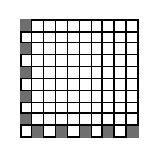
\includegraphics[scale=1.5]{Figs/Algorithms/sick}
\end{wrapfigure}

\medskip

Пример с диагональю может натолкнуть на неверный путь, когда пытаются доказать, что в начальный момент инфицированные клетки должны быть в каждой строке или столбце.
Но это далеко не так.
Например, при расположении инфицированных клеток, как показано на рисунке, заражается вся доска.

}

Существует великое множество способов заразить всю доску при помощи $n$ изначально инфицированных клеток, но, оказывается, нету способа сделать это с меньшим числом.
Здесь нужен магический параметр $P$, но какой?

Этот параметр --- периметр!
Когда клетка заражена, по меньшей мере, две из её сторон сливаются с внутренностью заражённой территории, и максимум две стороны добавляются к её границе.
Следовательно, периметр заражённой территории не может увеличиваться.
Поскольку периметр всей доски равен $4n$ (предполагая, что клетки единичные), начальная заражённая территория должна содержать минимум $n$ клеток.
\heart

Дополнительное упражнение для тех, кому интересно: докажите, что $n$ изначально инфицированных клеток необходимо даже тогда, когда верх и низ доски склеены так, что получился цилиндр.
Если же ещё склеить правую и левую стороны так, что получится тор, то достаточно (и необходимо) $n-1$ изначально инфицированных клеток.
Периметр здесь больше не поможет,
работает другой подход, найденный Брюсом Рихтером (университет Ватерлоо) %(Bruce Richter, University of Waterloo) 
и вашим автором.

\subsubsection*{Пустое ведро}% (EMPTYING A BUCKET)

Ещё одна красивая задача из бывшего Советского Союза, которая была представлена на V-й Всесоюзной математической олимпиаде в Риге в 1971 году.
Позже она появлялась (уже без хозяйственного инвентаря), на Математической олимпиаде Патнема 1983 года.
Задача попала ко мне от Кристиана Боргса из лабораторий «Microsoft Research». %(Christian Borgs of Microsoft Research).
Я покажу два решения --- одно моё, комбинаторное, и второе, элегантное, теоретико-числовое доказательство, найденное Сванте Янсоном из Уппсальского университета, Швеция %(Svante Janson of Uppsala University, Sweden)
(а также независимо от него, Гартом Пэйном). %(Garth Payne)).
Я не знаю, которое из двух решений, если не третье, предполагалось изначально.

\medskip

В решении Сванте, за параметр $P$ берётся содержимое конкретного ведра и показывается, как можно каждый раз уменьшать $P$ и довести его до нуля.
В моём доказательстве, напротив, показывается, как можно каждый раз \emph{увеличивать} $P$ до тех пор, пока одно из \emph{оставшихся} вёдер не окажется пустым.

Чтобы доказать последнее утверждение, во-первых, отметим, что можно предположить, что только одно из вёдер содержит нечётное число унций жидкости.
Действительно, если нету «нечётных» вёдер, то можно изменить шкалу, разделив объёмы на степень двойки.
Если же имеется больше двух «нечётных» вёдер, то первый же шаг с двумя из них сократит их число до одного или нуля.

Во-вторых, заметим, что с нечётным и чётным ведром всегда можно сделать \emph{обратный ход}, то есть вылить половину содержимого чётного ведра в нечётное.
Действительно, каждое состояние этой пары вёдер может быть достигнуто максимум из одного состояния, таким образом, после достаточного числа шагов вы пройдёте по циклу и вернётесь в начальное состояние.
Состояние \emph{прямо перед} тем, как вы возвращаетесь к начальному, и является результатом вашего «обратного хода».

И последнее, мы утверждаем, что, пока нет пустого ведра, содержимое нечётного ведра всегда можно увеличить.
Если есть ведро, у которого число унций содержимого делится на 4, то обратным ходом можно половину его перелить в нечётное ведро.
Если же такового нет, то его легко получить, совершив одну операцию между двумя чётными вёдрами.
\heart

А вот доказательство Сванте, в его собственном изложении:

\medskip

«Обозначим число унций жидкости, которое изначально содержалось в вёдрах $A$, $B$ и $C$ через $a$, $b$ и $c$, где $0<a\le b\le c$.
Я опишу последовательность шагов, приводящую к тому, что минимальный из трёх объёмов жидкости станет меньше, чем $a$.
Если минимум равен нулю, то задача решена; в противном случае, мы переобозначаем вёдра и повторяем процедуру.

Пусть $b = qa + r$, где $0\le r<a$ и $q\ge 1$ --- целое число.
Запишем $q$ в двоичной системе: $q=q_0+2q_1+\dots+2^nq_n$, где каждое $q_i$ это $0$ или $1$, и $q_n = 1$.

Проделаем $n+1$ шаг, пронумеровав их $0,\dots, n$ следующим образом: на $i$-м шаге  мы выливаем из $B$ в $A,$ если $q_i = 1$, и из $C$ в $A$, если $q_i = 0$.
Поскольку мы всё время льём в $A$, его содержимое каждый раз удваивается, так что $A$ содержит $2^ia$ перед $i$-м шагом.
Отсюда общий объём жидкости, вылитый из $B$ равен $qa$, таким образом, в конце $b-qa=r<a$ остаётся в $B$.
Заметим, что общий объём жидкости, вылитый из $C$ равен, максимум
\[\sum_{i=0}^{n-1} 2^ia<2^na\le qa\le b\le c.\]
Таким образом, в $C$ (и в $B$) достаточно жидкости, чтобы проделать все эти шаги.»
\heart

Насколько мне известно, никто не знает даже приблизительно, сколько требуется шагов для решения этой задачи (в худшем начальном состоянии с общим объёмом жидкости равным $n$ унциям).
Моё решение показывает, что достаточно порядка $n^2$ шагов.
Свантевское  решение лучше, оно ограничивает число шагов произведением константы на $n\log n$.
Окончательный ответ может оказаться ещё меньше.

\subsubsection*{Фишки по углам}% (PEGS ON THE CORNERS)

На эту симпатичную задачу обратил моё внимание Миккель Торуп из лабораторий AT\&T, %(Mikkel Thorup of AT&T Labs),
который её услышал от Ассафа Наора %(Assaf Naor)
(в то время научного сотрудника Майкрософта), который услышал её от аспирантов Еврейского университета в Иерусалиме.

\medskip

Заметим, что если фишки начинают ходить с вершин решётки (то есть точек плоскости с целыми координатами), то они всегда будут оставаться в вершинах решётки.

В частности, если изначально они располагаются в вершинах единичного квадрата решётки, то они, разумеется, не могут позже оказаться в углах \emph{меньшего} квадрата, поскольку в решётке не существует квадратов, меньше единичного.
Но почему не в углах б\'{о}льшего квадрата?

Основное наблюдение: прыжок через фишку обратим!
Если бы было возможно прийти к б\'{о}льшему квадрату, то мы могли бы обратить весь процесс и завершить ход на меньшем квадрате, что, как мы уже знаем, невозможно.
\heart

\subsubsection*{Фишки на полуплоскости}% (PEGS ON THE HALF-PLANE)

Это вариант задачи, описанной во втором томе «Выигрышных стратегий ваших математических игр».\footnote{E. Berlekamp, J. Conway, R. Guy,
\emph{Winning Ways for your Mathematical Plays.} Academic Press, 1982.}
Мы полагаем, задача была изначально придумана одним из авторов книги, Джоном Конвеем.
В его варианте не разрешались прыжки по диагонали, тем не менее, можно было без особых трудностей продвинуть фишку до линии $y = 4$.
Рассуждение, подобное приведённому ниже, показывает, что позиции выше достичь невозможно.

\medskip

С прыжками по диагонали или без, трудность состоит в том, что когда фишки поднимаются выше, вершины решётки под ними оголяются.
Нам нужен такой параметр $P$, который бы получал награду за ушедшую высоко фишку, но для компенсации подвергался бы наказанию за оставленные позади дырки.
Естественным выбором была бы сумма по всем фишкам некоторой функции от их позиции.
Поскольку фишек бесконечно много, необходимо позаботиться, чтобы сумма сходилась.

Например, фишке на $(0, y)$ можно присвоить вес $r^y$, где $r$ --- некое вещественное число большее $1$.
Так, что веса фишек на нижней части оси $Y$ в сумме дадут конечное число $\sum_{y\le 0}r^y = r/(r-1)$.
Веса в прилегающих столбцах нужно будет уменьшать, чтобы сумма по всей плоскости оставалась конечной.
Если на каждом шаге при удалении от оси $Y$ мы делим вес на $r$, то получаем, что вес фишки в точке $(x, y)$ равен $r^{y - |x|}$, и тогда общий вес в начальной позиции 
\[\frac r{r-1} + \frac 1{r-1} +\frac 1{r-1} +\frac 1{r(r-1)} +\frac 1{r(r-1)} + \dots =\frac{r^2+r}{(r-1)^2} <\infty.\]

Если фишка прыгнула, то в лучшем случае (когда прыжок был совершён по диагонали вверх к оси $Y$), $P$ приобретает $vr^4$ и теряет $v+vr^2$, где $v$ --- вес фишки перед прыжком.
Пока $r$ не превышает квадратный корень \emph{золотого сечения} $\varphi=(1+\sqrt5)/2\approx 1{,}618$, удовлетворяющего уравнению $\varphi^2=\varphi+1$, этот прирост не может быть положительным.

Далее, если положить $r = \sqrt{\varphi}$, то начальное значение $P$ составит примерно $39{,}0576$, но вес одной фишки в точке $(0, 16)$ \emph{сам по себе} равен $\varphi^8\approx 46{,}9788$.
Поскольку мы не можем увеличить $P$, то, следовательно, мы не можем продвинуть фишку на точку $(0, 16)$.

Но если бы мы смогли продвинуть фишку на \emph{любую} точку линии $y = 16$ или выше, то мы бы смогли попасть и в точку $(0, 16)$, остановив фишку, дошедшую до точки $(x, 16)$, и, повторив те же шаги на поле, сдвинутом вправо или влево на~$|x|$.
\heart

{\sloppy 

Нам неизвестно наибольшее значение $y$-координаты точки, до которой может дойти фишка при разрешённых диагональных прыжках.
Вполне возможно, какой-нибудь трудолюбивый читатель сможет устранить этот пробел.

}

\subsubsection*{Фишки на квадрате}% (PEGS IN A SQUARE)

Существует несколько способов решения данной задачи, которая является \emph{частью} задачи, представленной на Международной Математической Олимпиаде 1993 года.
Приведённое ниже доказательство мне рассказал Бенни Судаков из Принстонского университета.

\medskip

Покрасим вершины $(x, y)$ решётки в серый цвет, если ни $x$, ни $y$ не делятся на $3$, в противном случае --- в белый цвет.
Получается периодический узор из серых квадратов $2\times 2$ (см. рисунок). 

Если две соседние (ортогонально) фишки стоят обе в серых вершинах решётки или обе в белых, то фишка, оставшаяся после прыжка, окажется в белой вершине.
Если же одна вершина серая, а другая белая, то, напротив, фишка, оставшаяся после прыжка, будет стоять в серой вершине.
Из этого следует, что если изначально в серых вершинах находится чётное число фишек, то это свойство будет сохраняться.

\begin{figure}[h!]
\centering
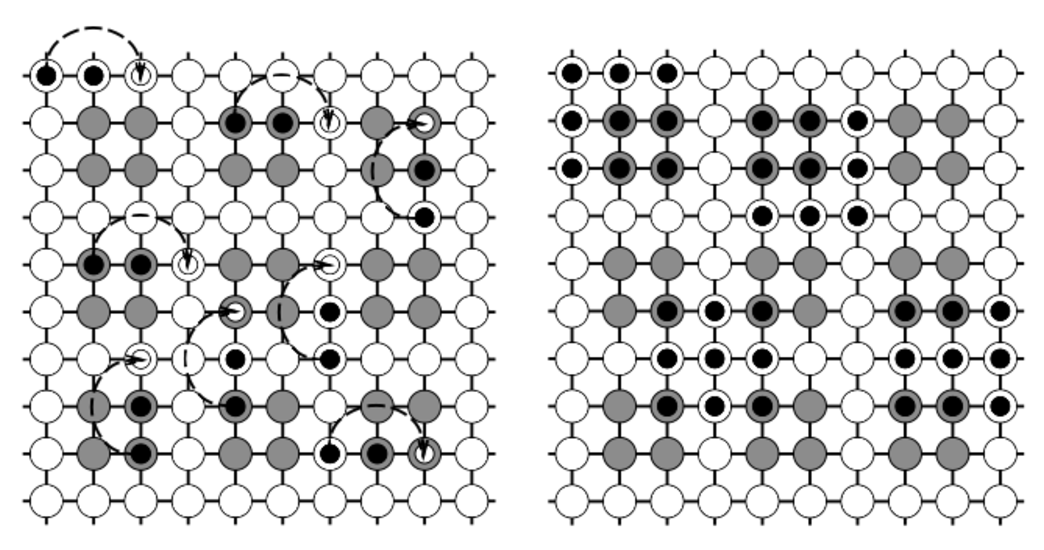
\includegraphics[scale=0.5]{Figs/Algorithms/square}
\end{figure}

Несложно увидеть, что если взять квадрат с фишками $3\times 3$ и поместить его на плоскость, то в какое бы место решётки мы его не определили, он всегда накроет чётное число серых вершин.
А так как квадрат $n\times n$, где $n$ кратно $3$, состоит из подобных квадратов, то в нём также всегда будет содержаться чётное число серых вершин.
Предположим, что оказалось возможным уменьшить число фишек в таком квадрате до одной.
Тогда мы смогли бы передвинуть начальный квадрат так, чтобы выжившая фишка оказалась в серой вершине. 
Это противоречие завершает доказательство.
\heart

Есть довольно техническое, не особенно простое и некрасивое, 
доказательство того, что если $n$ \emph{не} делится на $3$, то \emph{возможно} уменьшить число фишек до одной.
На олимпиаде участников просили точно определить, при каких $n$ квадраты можно свести к одной фишке --- довольно сурово требовать сделать это вот так сразу!

\subsubsection*{Кульбиты многоугольника}% (FLIPPING THE POLYGON)

Данная головоломка является обобщением задачи, появлявшейся на Международной Математической Олимпиаде 1986 года (представленной, как мне говорили, составителем из восточной Германии) и впоследствии получившей название «Задача о пентагоне».

Задача имеет много решений.
Более того, её можно обобщить и дальше, от $n$-угольников до произвольных связных графов.
Однако, решение, приводимое ниже, выделяется среди прочих сочетанием элегантности и строгости доказательства.
Его придумали, независимо друг от друга, хотя бы два математика, один из них --- Бернар Шазель, профессор информатики Принстонского университета. %(Bernard Chazelle, Professor of Computer Science at Princeton University)

\medskip

Пусть $x(0),\dots,x(n-1)$ --- числа при вершинах, дающие в сумме $s > 0$, с индексами, взятыми по модулю $n$.
Определим двустороннюю бесконечную последовательность
$b(\cdot)$, где $b(0) = 0$ и $b(i) = b(i -1) + x(i \mod{n})$.
Последовательность $b(\cdot)$ не является периодической, но она периодически возрастает: $b(i + n) = b(i) + s$.

\begin{figure}
\centering
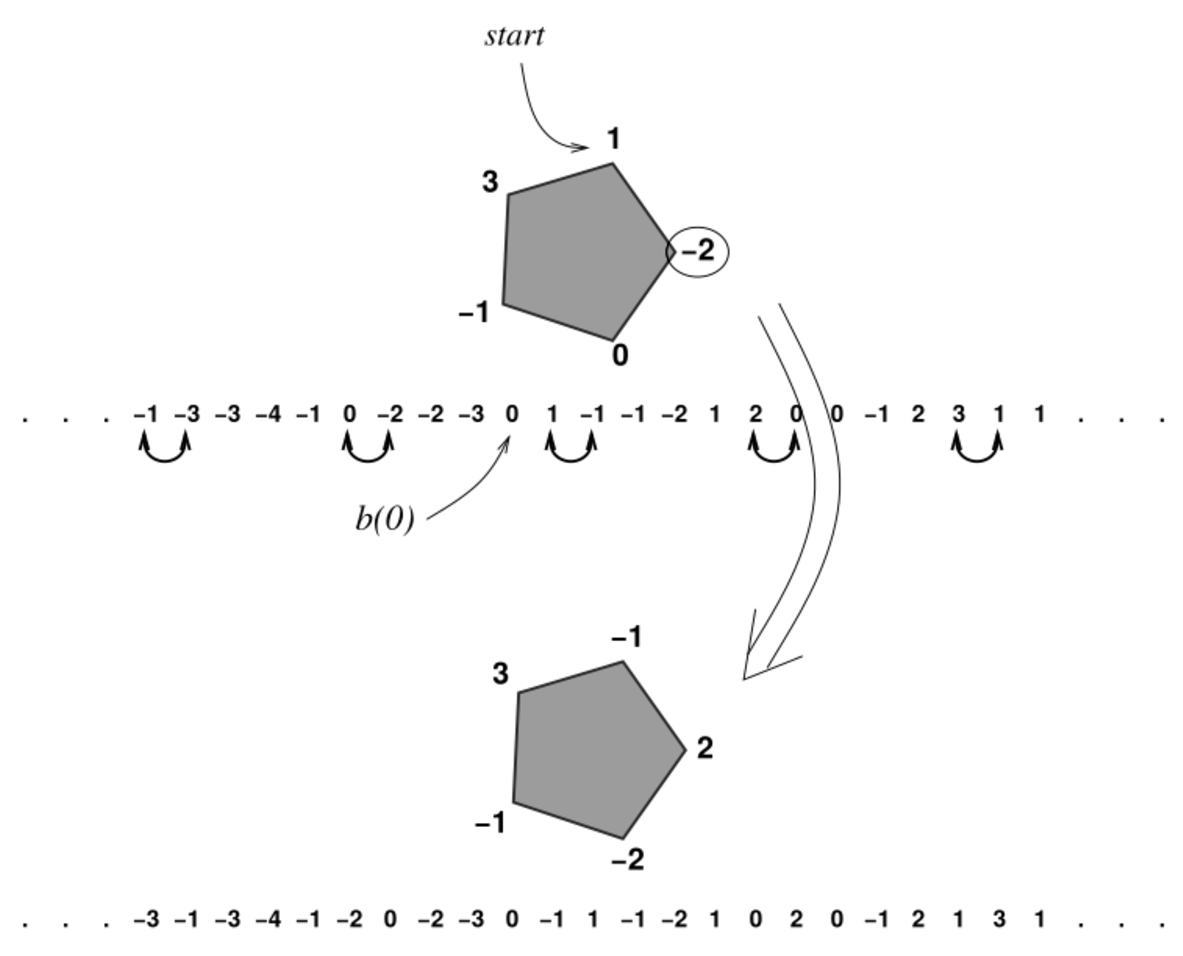
\includegraphics[scale=0.5]{Figs/Algorithms/sort}
\end{figure}

Если $x(i)$ --- отрицательно, то $b(i) < b(i-1)$, и, меняя знак у $x(i)$, получаем тот же эффект, как при замене $b(i)$ на $b(i - 1)$, так что они располагаются теперь в возрастающем порядке.
Это верно и для всех пар $b(j)$, $b(j - 1)$, сдвинутых на числа, кратные $n$.
Таким образом, изменение знака при вершине сводится к упорядочиванию $b(\cdot)$, используя перестановки соседних членов!

Чтобы проследить за ходом процесса сортировки, нам нужен некий конечный параметр $P$, который измеряет степень, при которой $b(\cdot)$ нарушает порядок. % (out of order).
Для нахождения его, положим $i^+$ --- число индексов $j > i$, для которых $b(j) < b(i)$, и $i^-$ --- число индексов $j < i$, для которых $b(j) > b(i)$.
Обратите внимание, что $i^+$ и $i^-$ имеют конечное значение и зависят только от $i \pmod n$.
Также отметим, что 
\[\sum_{i=0}^{n-1}i^+=\sum_{i=0}^{n-1}i^-\]
и пусть эта сумма будет нашим волшебным параметром $P$.

Когда $x(i+1)$ меняет знак, $i^+$ уменьшается на $1$, а все другие $j^+$ не меняются.
Значит, $P$ уменьшается \emph{в точности} на 1.
Когда $P$ достигает $0$, последовательность полностью отсортирована, так что все числа у вершин неотрицательны, и процесс прекращается.

Мы доказали больше, чем требовалось:
независимо от выбора чисел в этом процессе, он заканчивается за одно и тоже ($P$) число шагов,
более того, конечная конфигурация также не зависит от порядка выбора чисел!
Причина этого кроется в том, что существует только один способ сортировки $b(\cdot)$.
Когда сортировка завершена, член исходной последовательности $b(i)$ должен оказаться в позиции $i \z+ i^+ - i^-$.
\heart

\subsubsection*{Лампочки по кругу}% (LIGHT BULBS IN A CIRCLE)

Эта головоломка является частью задачи, представленной на Международной Математической Олимпиаде 1993 года.
При неуказанном значении $n$ лучшим способом решения будет показать (как мы это уже делали в одном из доказательств «Пустого ведра»), что само пространство состояний является циклическим.

\medskip

Во-первых, отметим, что нет опасности выключить все лампочки,
ведь если это изменение сделано в момент времени $t$, то лампочка номер $t$ всё ещё включена.

Более того, если мы посмотрим на наш круг сразу \emph{после} момента $t$, то узнаем, в каком состоянии были лампочки в момент~$t$ (изменив состояние лампочки $t+1$, если лампочка $t$ включена).
Поскольку число возможных состояний в круге конечно (мы учитываем, какая лампочка рассматривается, а также какие лампочки включены), то мы со временем должны будем повторить некое состояние в первый раз.
Скажем, в момент времени $t_1$ повторилось состояние, бывшее в момент $t_0$, где $t_1$ и $t_0$ отличаются на число, кратное $n$.
Но тогда в момент $t_1 - 1$ мы уже были в том же состоянии, как и в момент $t_0 - 1$, что является противоречием, если только момента $t_0 - 1$ не существовало.
А это значит, что $t_0=0$, то есть повторилось состояние, когда все лампочки были включены.
\heart

\subsubsection*{Жуки на многограннике}% (BUGS ON A POLYHEDRON)

Данная задача была представлена в статье Антона Клячко.%
\footnote{A. Klyachko, ``А Funny Property of Sphere and Equations over Groups''. \emph{Communications in Algebra}, Vol. 21, No. 7 (1993), 2555--2575.} 
Для её решения мы, по сути, должны сделать противоположное тому, что делали в предыдущей задаче, то есть показать, что некий параметр будет всегда меняться в одном направлении, и, таким образом, мы не сможем вернуться в исходное состояние.

\medskip

Заметим, что можно предположить, что в начальный момент ни один жук не стоит в вершине (можно жуков слегка подтолкнуть или придержать).
Можно также предположить, что, никакая пара жуков не проходит через вершины одновременно.

\begin{figure}[h!]
\centering
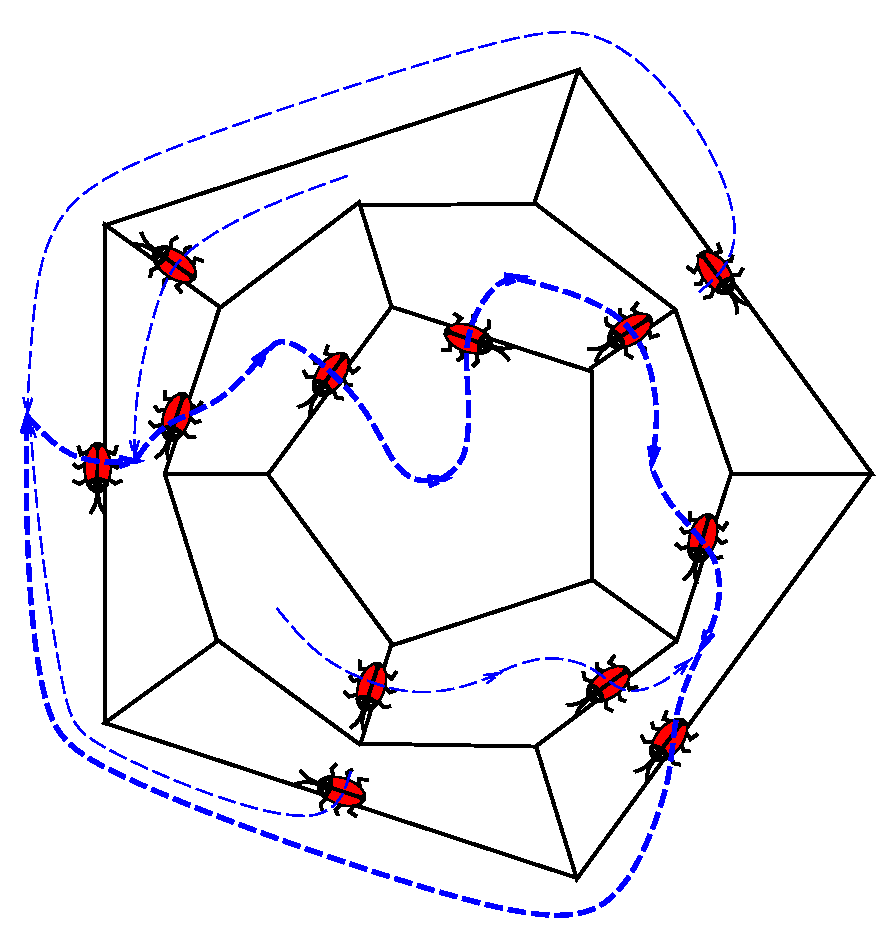
\includegraphics[scale=0.5]{Figs/Algorithms/dodec}
\end{figure}

В любой момент времени можно нарисовать стрелку из центра каждой грани $F$ к жуку с этой грани и дальше, к центру грани с другой стороны от жука.
Начав с любой грани и следуя далее по таким стрелкам, мы должны будем, в конце концов, оказаться на некой грани второй раз, завершив цикл стрелок на многограннике.

Этот цикл разделяет поверхность многогранника на две части.
Назовём внутренней частью цикла ту, которую мы обходим по часовой стрелке.
Обозначим через $P$ число вершин многогранника внутри цикла.

Изначально $P$ могло принимать любое значение от $0$ до числа всех (скажем, $n$) вершин многогранника.
Экстремальные значения получаются, когда два жука ползут по одному ребру, и, следовательно, длина цикла равна $2$.
В случае, когда $P=0$, два жука ползут по ребру навстречу друг другу, и столкновение неизбежно.

В момент, когда один из жуков в цикле переходит на следующее ребро, стрелка, проходящая через него, поворачивается вправо.
Вершина, через которую он переползает, бывшая до того внутри цикла, оказывается теперь снаружи.
Другие вершины также могли перейти из внутренней части цикла во внешнюю, но не существует способа перейти из внешней части во \emph{внутреннюю}.
Чтобы это увидеть, заметьте, что новая стрелка теперь направлена внутрь цикла.
У последовательности стрелок, исходящих из её конца, нет никакой возможности избежать зацикливания, они неизбежно придут к началу какой-то стрелки цикла, создав новый цикл с меньшей внутренней частью.
В частности, значение $P$ уменьшилось хотя бы на~$1$.

{

\sloppy

Поскольку $P$ не сможет принять своё начальное значение, нам остаётся только надеяться, что у жуков имеется страховка от несчастного случая.
\heart

}

\subsubsection*{Жуки на числовом луче}% (BUGS ON THE LINE)

Для начала нам нужно убедиться, что жук \emph{либо} свалится с левого конца луча, либо убежит на бесконечность вправо, то есть он не может вечно ползать туда-сюда.
Для этого ему пришлось бы проходить через какие-то числа бесконечное число раз.
Пусть $n$ --- наименьшее из таких чисел.
Здесь необходимо отметить, что попадая каждый третий раз на число $n$, жук увидит там красный свет, и следовательно, будет вынужден уползти влево на $n-1$, а это противоречит предположению, что он посетил $n-1$ только конечное число раз.

Теперь, когда с этим всё ясно, будет полезным думать о зелёном свете, как о цифре 0, о красном, как о 1, и о жёлтом, как это ни парадоксально, как о «цифре» $\tfrac12$.
А расположение цветов лампочек может быть представлено как число между $0$ и $1$, записанное в двоичной системе
\[x = 0{,}\,x_1\,x_2\,x_3\dots;\]
то есть,
 \[x = x_1\cdot(\tfrac12)+x_2\cdot(\tfrac12)^2+\dots\]
Будем думать о жуке в точке $i$, как о дополнительной «1» к $i$-й позиции, определяемой как
\[y=x+(\tfrac12)^i.\]
Ключевое наблюдение состоит в том, что $y$ является \emph{инвариантом}, то есть его значение не меняется при передвижении жука.
Если жук идёт вправо от точки $i$, то значение числа, на котором он сидел, поднимается на $\tfrac12$.
Следовательно, $x$ увеличивается на $(\tfrac12)^{i+1}$, а собственное значение жука уменьшается на ту же самую величину.
Если жук идёт налево от $i$, он увеличивает своё значение на $(\tfrac12)^i$ и это компенсируется тем, что значение $x$ уменьшается на целую цифру в $i$-й позиции.

Исключение составляет только момент, когда жук сваливается с левого конца луча.
В этом случае и $x$, и собственное значение жука уменьшаются на $\tfrac12$, то есть общая потеря равна $1$.
Когда выставляется следующий жук, $y$ увеличивается на $\tfrac12$.
Другими словами, значение $x$ поднимается на $\tfrac12$, если выставляется новый жук, и он исчезает справа на бесконечности; и $x$ падает на $\tfrac12$, если выставляется новый жук, и он сваливается с левого конца луча.

Конечно же, в любой момент $x$ должен лежать в единичном интервале.
Если его начальное значение лежит строго между $0$ и $\tfrac12$, то жуки должны будут поочерёдно убегать направо, падать слева, убегать, падать и так далее.
Если же $x$ лежит строго между $\tfrac12$ и $1$, то жуки поочерёдно будут падать, убегать, падать, убегать и так далее.

Оставшиеся случаи можно проверить руками.
Если изначально $x = 1$ (все точки --- красные), первый жук переключит $1$ на зелёный и свалится слева.
Второй жук, вихляя, удаляется вправо на бесконечность, оставив все лампочки опять красными, то есть мы получим чередование: падает, убегает, падает, убегает...

Если $x = 0$ (то есть все точки --- зелёные), то первый жук убежит, второй опять убежит (так как все точки сменятся на жёлтые, а потом на все красные), а затем чередование --- падает, убегает, падает, убегает..., как и прежде.

Самый интересный случай --- это $x=\tfrac12$, так как существует несколько способов представления $\tfrac12$ в нашей модифицированной двоичной системе: $x$ может быть составлен из одних $\tfrac12$, или он может начинаться с любого конечного числа (включая ноль) $\tfrac12$, за которым следуют либо $0111\dots$, либо $1000\dots$.
В первом случае начинающий жук переключит все жёлтые лампочки на красные по мере удаления направо, таким образом, мы получаем чередование  убегает, падает, убегает, падает...
Второй случай такой же, первый жук, вихляя, уползает направо, опять оставляя все точки после себя красными.
В третьем случае жук переключает жёлтый на красный по ходу движения, но когда он достигает красной точки, он разворачивается и двигается налево, меняя красный на зелёный по пути, пока не свалится с конца луча.
После этого приходим к случаю $x = 0$, так что в этом случае  последовательность будет: падает, убегает, падает, убегает...

Возвращаясь опять ко всем случаям, мы видим, что всякий раз, когда второй жук падает, третий жук убегает.
\heart

Это элегантное рассуждение представили
Анде Холройд (Университет Британской Колумбии) и Джим Пропп (Висконсинский университет) на встрече группы «Институт Элементарных Исследований» в Баннфе, Альберта в 2003 году. %
%\footnote{прим. перев.: \href{https://www.birs.ca/files/scientific-reports/}{\url{www.birs.ca/files/scientific-reports/BIRS_SR_2003.pdf}} стр. 63}
Пропп предложил использовать жука, чтобы детерминизированно смоделировать случайные блуждания на неотрицательных целых числах, в которых шаги делаются (независимо) влево с вероятностью $\tfrac13$ и вправо с вероятностью $\tfrac23$.
В подобных блужданиях конкретный жук падает с левого конца луча или убегает на бесконечность вправо с одинаковой вероятностью.
Но как мы видели, детерминизированная модель показывает вместо этого, что после первой пары жуков направления строго чередуются.
Доказательство может быть обобщено и на другие виды случайных блужданий.

\subsubsection*{Как разломать шоколадку}% (BREAKING A CHOCOLATE BAR)

Эта до смешного простая задача известна тем, что некоторые \emph{очень} крутые математики зависали на ней на целый день, пока среди  стенаний и битья головой об стену на них не снисходило озарение.
Рискуя прослыть садистом, я пропускаю доказательство.
